% Options for packages loaded elsewhere
\PassOptionsToPackage{unicode}{hyperref}
\PassOptionsToPackage{hyphens}{url}
\PassOptionsToPackage{dvipsnames,svgnames,x11names}{xcolor}
%
\documentclass[
  a4paper,
]{scrreport}

\usepackage{amsmath,amssymb}
\usepackage{iftex}
\ifPDFTeX
  \usepackage[T1]{fontenc}
  \usepackage[utf8]{inputenc}
  \usepackage{textcomp} % provide euro and other symbols
\else % if luatex or xetex
  \usepackage{unicode-math}
  \defaultfontfeatures{Scale=MatchLowercase}
  \defaultfontfeatures[\rmfamily]{Ligatures=TeX,Scale=1}
\fi
\usepackage{lmodern}
\ifPDFTeX\else  
    % xetex/luatex font selection
\fi
% Use upquote if available, for straight quotes in verbatim environments
\IfFileExists{upquote.sty}{\usepackage{upquote}}{}
\IfFileExists{microtype.sty}{% use microtype if available
  \usepackage[]{microtype}
  \UseMicrotypeSet[protrusion]{basicmath} % disable protrusion for tt fonts
}{}
\makeatletter
\@ifundefined{KOMAClassName}{% if non-KOMA class
  \IfFileExists{parskip.sty}{%
    \usepackage{parskip}
  }{% else
    \setlength{\parindent}{0pt}
    \setlength{\parskip}{6pt plus 2pt minus 1pt}}
}{% if KOMA class
  \KOMAoptions{parskip=half}}
\makeatother
\usepackage{xcolor}
\setlength{\emergencystretch}{3em} % prevent overfull lines
\setcounter{secnumdepth}{5}
% Make \paragraph and \subparagraph free-standing
\makeatletter
\ifx\paragraph\undefined\else
  \let\oldparagraph\paragraph
  \renewcommand{\paragraph}{
    \@ifstar
      \xxxParagraphStar
      \xxxParagraphNoStar
  }
  \newcommand{\xxxParagraphStar}[1]{\oldparagraph*{#1}\mbox{}}
  \newcommand{\xxxParagraphNoStar}[1]{\oldparagraph{#1}\mbox{}}
\fi
\ifx\subparagraph\undefined\else
  \let\oldsubparagraph\subparagraph
  \renewcommand{\subparagraph}{
    \@ifstar
      \xxxSubParagraphStar
      \xxxSubParagraphNoStar
  }
  \newcommand{\xxxSubParagraphStar}[1]{\oldsubparagraph*{#1}\mbox{}}
  \newcommand{\xxxSubParagraphNoStar}[1]{\oldsubparagraph{#1}\mbox{}}
\fi
\makeatother


\providecommand{\tightlist}{%
  \setlength{\itemsep}{0pt}\setlength{\parskip}{0pt}}\usepackage{longtable,booktabs,array}
\usepackage{calc} % for calculating minipage widths
% Correct order of tables after \paragraph or \subparagraph
\usepackage{etoolbox}
\makeatletter
\patchcmd\longtable{\par}{\if@noskipsec\mbox{}\fi\par}{}{}
\makeatother
% Allow footnotes in longtable head/foot
\IfFileExists{footnotehyper.sty}{\usepackage{footnotehyper}}{\usepackage{footnote}}
\makesavenoteenv{longtable}
\usepackage{graphicx}
\makeatletter
\def\maxwidth{\ifdim\Gin@nat@width>\linewidth\linewidth\else\Gin@nat@width\fi}
\def\maxheight{\ifdim\Gin@nat@height>\textheight\textheight\else\Gin@nat@height\fi}
\makeatother
% Scale images if necessary, so that they will not overflow the page
% margins by default, and it is still possible to overwrite the defaults
% using explicit options in \includegraphics[width, height, ...]{}
\setkeys{Gin}{width=\maxwidth,height=\maxheight,keepaspectratio}
% Set default figure placement to htbp
\makeatletter
\def\fps@figure{htbp}
\makeatother

%\newfontfamily\Ubuntu[Mapping=tex-text]{Ubuntu}
\usepackage{pgfplots}
\usetikzlibrary{arrows.meta,arrows}
\usetikzlibrary{angles,quotes}
\pgfplotsset{grid style={dashed,mygray}}
% Colors
\definecolor{myblue}{rgb}{0.067,0.529,0.871}
\definecolor{mypurple}{rgb}{0.859,0.071,0.525}
\definecolor{myred}{rgb}{1.0, 0.13, 0.32}
\definecolor{mygreen}{rgb}{0.01, 0.75, 0.24}
\definecolor{myblack}{gray}{0.1}
\definecolor{mygray}{gray}{0.8}
\newcommand{\NN}{\mathbb{N}}
\newcommand{\ZZ}{\mathbb{Z}}
\newcommand{\QQ}{\mathbb{Q}}
\newcommand{\RR}{\mathbb{R}}
\newcommand{\CC}{\mathbb{C}}
\DeclareMathOperator{\operatorname{Int}}{Int}
\DeclareMathOperator{\operatorname{Ext}}{Ext}
\DeclareMathOperator{\operatorname{Fr}}{Fr}
\DeclareMathOperator{\Adh}{Adh}
\DeclareMathOperator{\Ac}{Ac}
\DeclareMathOperator{\sen}{sen}
\makeatletter
\@ifpackageloaded{tcolorbox}{}{\usepackage[skins,breakable]{tcolorbox}}
\@ifpackageloaded{fontawesome5}{}{\usepackage{fontawesome5}}
\definecolor{quarto-callout-color}{HTML}{909090}
\definecolor{quarto-callout-note-color}{HTML}{0758E5}
\definecolor{quarto-callout-important-color}{HTML}{CC1914}
\definecolor{quarto-callout-warning-color}{HTML}{EB9113}
\definecolor{quarto-callout-tip-color}{HTML}{00A047}
\definecolor{quarto-callout-caution-color}{HTML}{FC5300}
\definecolor{quarto-callout-color-frame}{HTML}{acacac}
\definecolor{quarto-callout-note-color-frame}{HTML}{4582ec}
\definecolor{quarto-callout-important-color-frame}{HTML}{d9534f}
\definecolor{quarto-callout-warning-color-frame}{HTML}{f0ad4e}
\definecolor{quarto-callout-tip-color-frame}{HTML}{02b875}
\definecolor{quarto-callout-caution-color-frame}{HTML}{fd7e14}
\makeatother
\makeatletter
\@ifpackageloaded{bookmark}{}{\usepackage{bookmark}}
\makeatother
\makeatletter
\@ifpackageloaded{caption}{}{\usepackage{caption}}
\AtBeginDocument{%
\ifdefined\contentsname
  \renewcommand*\contentsname{Tabla de contenidos}
\else
  \newcommand\contentsname{Tabla de contenidos}
\fi
\ifdefined\listfigurename
  \renewcommand*\listfigurename{Listado de Figuras}
\else
  \newcommand\listfigurename{Listado de Figuras}
\fi
\ifdefined\listtablename
  \renewcommand*\listtablename{Listado de Tablas}
\else
  \newcommand\listtablename{Listado de Tablas}
\fi
\ifdefined\figurename
  \renewcommand*\figurename{Figura}
\else
  \newcommand\figurename{Figura}
\fi
\ifdefined\tablename
  \renewcommand*\tablename{Tabla}
\else
  \newcommand\tablename{Tabla}
\fi
}
\@ifpackageloaded{float}{}{\usepackage{float}}
\floatstyle{ruled}
\@ifundefined{c@chapter}{\newfloat{codelisting}{h}{lop}}{\newfloat{codelisting}{h}{lop}[chapter]}
\floatname{codelisting}{Listado}
\newcommand*\listoflistings{\listof{codelisting}{Listado de Listados}}
\usepackage{amsthm}
\theoremstyle{definition}
\newtheorem{exercise}{Ejercicio}[chapter]
\theoremstyle{remark}
\AtBeginDocument{\renewcommand*{\proofname}{Prueba}}
\newtheorem*{remark}{Observación}
\newtheorem*{solution}{Solución}
\newtheorem{refremark}{Observación}[chapter]
\newtheorem{refsolution}{Solución}[chapter]
\makeatother
\makeatletter
\makeatother
\makeatletter
\@ifpackageloaded{caption}{}{\usepackage{caption}}
\@ifpackageloaded{subcaption}{}{\usepackage{subcaption}}
\makeatother

\ifLuaTeX
\usepackage[bidi=basic]{babel}
\else
\usepackage[bidi=default]{babel}
\fi
\babelprovide[main,import]{spanish}
% get rid of language-specific shorthands (see #6817):
\let\LanguageShortHands\languageshorthands
\def\languageshorthands#1{}
\ifLuaTeX
  \usepackage{selnolig}  % disable illegal ligatures
\fi
\usepackage{bookmark}

\IfFileExists{xurl.sty}{\usepackage{xurl}}{} % add URL line breaks if available
\urlstyle{same} % disable monospaced font for URLs
\hypersetup{
  pdftitle={Problemas de Estadística},
  pdfauthor={Alfredo Sánchez Alberca},
  pdflang={es},
  colorlinks=true,
  linkcolor={blue},
  filecolor={Maroon},
  citecolor={Blue},
  urlcolor={Blue},
  pdfcreator={LaTeX via pandoc}}


\title{Problemas de Estadística}
\author{Alfredo Sánchez Alberca}
\date{2022-01-06}

\begin{document}
\begin{titlepage}

%\AddToShipoutPicture*{\put(0,0){\includegraphics[scale=0.8]{img/background2}}} % Imagen de fondo, requiere el paquete eso-pic.
\begin{center}
\vspace*{5cm}

\Huge
{\textbf{\textsf{Problemas de Estadística}}}

\vspace{0.5cm}
\LARGE
{\textbf{\textsf{}}}

\vspace{1.5cm}

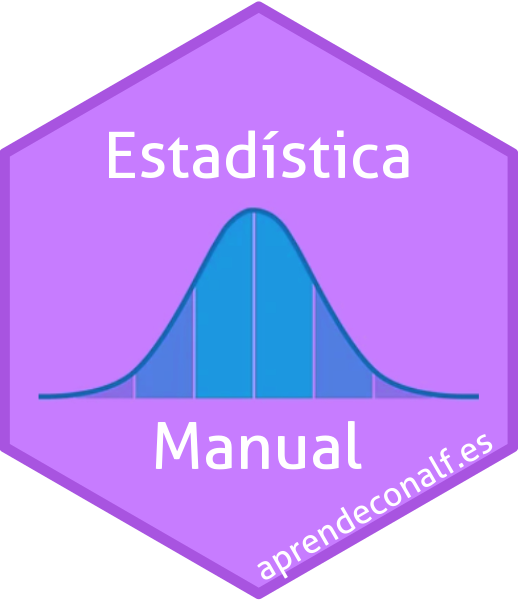
\includegraphics[width=0.4\textwidth]{img/logos/sticker.png}
\end{center}

\vfill

\begin{flushleft}
\begin{tabular}{ll}

\includegraphics[width=0.1\textwidth]{img/logos/aprendeconalf.png} & \parbox[b]{5cm}{\Large\textsf{Alfredo
Sánchez
Alberca}\\ \textsf{asalber@ceu.es} \\ \textsf{https://aprendeconalf.es}}
\end{tabular}
\end{flushleft}
\end{titlepage}
\renewcommand*\contentsname{Tabla de contenidos}
{
\hypersetup{linkcolor=}
\setcounter{tocdepth}{2}
\tableofcontents
}

\bookmarksetup{startatroot}

\chapter*{Prefacio}\label{prefacio}
\addcontentsline{toc}{chapter}{Prefacio}

\markboth{Prefacio}{Prefacio}

Colección de problemas de Estadística aplicada a la Economía para el
Master en Análisis y Comunicación de Datos.

\bookmarksetup{startatroot}

\chapter{Estimación de parámetros}\label{estimaciuxf3n-de-paruxe1metros}

\begin{exercise}[]\protect\hypertarget{exr-distribución-media-trabajadores-pymes}{}\label{exr-distribución-media-trabajadores-pymes}

El número medio de trabajadores en las PYMES españolas es \(5\) y su
varianza \(4\). Realizado un muestreo aleatorio de \(16\) PYMES,
calcular:

\begin{enumerate}
\def\labelenumi{\alph{enumi}.}
\item
  La esperanza y varianza de la media muestral.
\item
  La esperanza de la varianza y de la cuasivarianza muestral.
\item
  Mínimo tamaño que ha de tener la muestra para que exista una
  probabilidad mayor o igual al \(95\)\% de que la media muestral se
  desvíe de la media poblacional a lo sumo \(0.5\) unidades.
\item
  Si realizamos un muestreo aleatorio de tamaño \(320\) obtener
  \(P(4.9\leq \bar x  \leq 5.2)\).
\end{enumerate}

\end{exercise}

\begin{tcolorbox}[enhanced jigsaw, colframe=quarto-callout-tip-color-frame, breakable, opacityback=0, titlerule=0mm, opacitybacktitle=0.6, bottomtitle=1mm, toptitle=1mm, colback=white, leftrule=.75mm, colbacktitle=quarto-callout-tip-color!10!white, arc=.35mm, rightrule=.15mm, left=2mm, bottomrule=.15mm, toprule=.15mm, title=\textcolor{quarto-callout-tip-color}{\faLightbulb}\hspace{0.5em}{Solución}, coltitle=black]

Sea \(X\) la variable aleatoria que mide el número de trabajadores en
una muestra de 16 PYMES españolas.

\begin{enumerate}
\def\labelenumi{\alph{enumi}.}
\tightlist
\item
  \(E(\bar x) = 5\) y \(Var(\bar x) = \frac{4}{16} = 0.25\).
\item
  \(E(s^2) = 3.75\) y \(E(\hat s^2) = 4\).
\item
  \(P(|\bar x - 5| \leq 0.5) = 0.95\) si \(n\geq 320\).
\item
  Sea \(Y\) la variable aleatoria que mide el número de trabajadores en
  una muestra de 320 PYMES españolas. Entonces,
  \(Y\sim N\left(5, \sqrt{\frac{4}{320}}\right)\) y
  \(P(4.9\leq \bar x  \leq 5.2) = 0.777\).
\end{enumerate}

\end{tcolorbox}

\begin{exercise}[]\protect\hypertarget{exr-distribución-cuasivarianza-iberpapel}{}\label{exr-distribución-cuasivarianza-iberpapel}

El precio de las acciones de Iberpapel se distribuyen según un modelo
normal \(N(\mu, 2)\). Si se analizan \(16\) sesiones de la Bolsa de
Madrid elegidas aleatoriamente, ¿cuál es la probabilidad de que la
cuasivarianza muestral del precio de las acciones sea mayor o igual que
\(2.136\)?

\end{exercise}

\begin{tcolorbox}[enhanced jigsaw, colframe=quarto-callout-tip-color-frame, breakable, opacityback=0, titlerule=0mm, opacitybacktitle=0.6, bottomtitle=1mm, toptitle=1mm, colback=white, leftrule=.75mm, colbacktitle=quarto-callout-tip-color!10!white, arc=.35mm, rightrule=.15mm, left=2mm, bottomrule=.15mm, toprule=.15mm, title=\textcolor{quarto-callout-tip-color}{\faLightbulb}\hspace{0.5em}{Solución}, coltitle=black]

Sabemos que \(\frac{ns^2}{\sigma^2}\sim \chi^2(n-1)\). Por tanto,
\(P(\hat s^2\geq 2.136) = P\left(\frac{16\cdot s^2}{2}\geq 4\cdot 2.136\right) = P\left(\chi^2(15)\geq 8.544\right) = 0.9\).

\end{tcolorbox}

\begin{exercise}[]\protect\hypertarget{exr-diferencia-proporciones-votos}{}\label{exr-diferencia-proporciones-votos}

El porcentaje de votantes con preferencia de un determinado partido es
del \(5\)\% en una región \(A\), y el \(10\)\% en otra \(B\).
Consultados \(100\) electores de la región \(A\) y \(150\) de la \(B\),
determinar la probabilidad de que el porcentaje de electores consultados
favorables a dicho partido en la segunda región supere en más de \(2\)\%
al porcentaje de electores favorables a dicho partido en la primera.

\end{exercise}

\begin{tcolorbox}[enhanced jigsaw, colframe=quarto-callout-tip-color-frame, breakable, opacityback=0, titlerule=0mm, opacitybacktitle=0.6, bottomtitle=1mm, toptitle=1mm, colback=white, leftrule=.75mm, colbacktitle=quarto-callout-tip-color!10!white, arc=.35mm, rightrule=.15mm, left=2mm, bottomrule=.15mm, toprule=.15mm, title=\textcolor{quarto-callout-tip-color}{\faLightbulb}\hspace{0.5em}{Solución}, coltitle=black]

Sea \(X_1\) proporción de votantes favorables al partido en la región
\(A\) en una muestra de \(100\) electores y \(X_2\) proporción de
votantes favorables al partido en la región \(B\) en una muestra de
\(150\) electores. Entonces,
\(X_1\sim N\left(0.05, \sqrt{\frac{0.05\cdot (1-0.05)}{100}}\right)\) y
\(X_2\sim N\left(0.1, \sqrt{\frac{0.1\cdot (1-0.1)}{150}}\right)\), y
\(P(X_2-X_1>0.02) = 0.8212\).

\end{tcolorbox}

\begin{exercise}[]\protect\hypertarget{exr-intervalo-confianza-media-carne-porcino}{}\label{exr-intervalo-confianza-media-carne-porcino}

Se sabe que el gasto mensual en carne de porcino en las familias
españolas se distribuye de manera normal. Se ha realizado un muestreo
aleatorio simple en el que se ha preguntado a \(20\) familias sobre el
gasto mensual en carne de porcino, y se ha obtenido una media de
\(170.31\) € y una cuasidesviación típica de \(36\) €.

\begin{enumerate}
\def\labelenumi{\alph{enumi}.}
\item
  Obtener el intervalo de confianza para el gasto medio mensual en carne
  de porcino con un 95\% de confianza.
\item
  ¿Cómo podría obtenerse un intervalo de confianza más preciso para el
  gasto medio suponiendo que no varían la media muestral, la
  cuasivarianza muestral y el tamaño de la muestra? ¿Y si no varían la
  media muestral, la cuasivarianza muestral y el nivel de confianza?
\item
  Obtener el intervalo de confianza para la desviación típica del gasto
  mensual en carne de porcino con un 95\% de confianza.
\end{enumerate}

\end{exercise}

\begin{tcolorbox}[enhanced jigsaw, colframe=quarto-callout-tip-color-frame, breakable, opacityback=0, titlerule=0mm, opacitybacktitle=0.6, bottomtitle=1mm, toptitle=1mm, colback=white, leftrule=.75mm, colbacktitle=quarto-callout-tip-color!10!white, arc=.35mm, rightrule=.15mm, left=2mm, bottomrule=.15mm, toprule=.15mm, title=\textcolor{quarto-callout-tip-color}{\faLightbulb}\hspace{0.5em}{Solución}, coltitle=black]

Sea \(X\sim N(\mu,\sigma)\) la variable aleatoria que mide el gasto
mensual en carne de porcino en una muestra de 20 familias españolas.

\begin{enumerate}
\def\labelenumi{\alph{enumi}.}
\item
  Usando el intervalo de confianza de la t de Student se tiene
  \(\mu \in (153.46, 187.16)\) con una confianza del \(95\)\%.
\item
  Para obtener un intervalo de confianza más preciso para el gasto medio
  manteniendo la misma media muestral, cuasivarianza muestral y tamaño
  de la muestra, se puede reducir el nivel de confianza.

  Y para obtener un intervalo de confianza más preciso para el gasto
  medio manteniendo la misma media muestral, cuasivarianza muestral y
  nivel de confianza, se puede aumentar el tamaño de la muestra.
\item
  Usando el intervalo de confianza de la \(\chi^2\) se tiene
  \(\sigma \in (27.37, 52.58)\) con una confianza del \(95\)\%.
\end{enumerate}

\end{tcolorbox}

\begin{exercise}[]\protect\hypertarget{exr-intervalo-confianza-media-peso}{}\label{exr-intervalo-confianza-media-peso}

La OMS ha obtenido una muestra de los pesos de \(50\) niños de \(12\)
años, que proporciona una media muestral de \(47\) kg y una
cuasidesviación típica muestral de \(11\) kg. Suponiendo que la
población sigue una distribución normal:

\begin{enumerate}
\def\labelenumi{\alph{enumi}.}
\item
  Obtener un intervalo de confianza para la media poblacional con un
  \(95\)\% de nivel de confianza.
\item
  El director de la OMS considera que el intervalo es poco preciso, pero
  quiere mantener el nivel de confianza. Por ello decide reducir a la
  mitad la amplitud del intervalo. En estas condiciones, ¿cuál debería
  ser el tamaño de la muestra para cumplir los objetivos del director?
\item
  Los resultados obtenidos en los análisis anteriores siguen sin
  convencer al director de la OMS y le pide a su equipo que establezca
  un intervalo de confianza para la media poblacional con un \(99\)\% de
  nivel de confianza, manteniendo la misma muestra del primer apartado.
\item
  El director decide reducir en un tercio la amplitud del intervalo
  anterior, pero quiere mantener el nivel de confianza ¿cuál debería ser
  el tamaño de la muestra para cumplir dicho objetivo?
\end{enumerate}

\end{exercise}

\begin{tcolorbox}[enhanced jigsaw, colframe=quarto-callout-tip-color-frame, breakable, opacityback=0, titlerule=0mm, opacitybacktitle=0.6, bottomtitle=1mm, toptitle=1mm, colback=white, leftrule=.75mm, colbacktitle=quarto-callout-tip-color!10!white, arc=.35mm, rightrule=.15mm, left=2mm, bottomrule=.15mm, toprule=.15mm, title=\textcolor{quarto-callout-tip-color}{\faLightbulb}\hspace{0.5em}{Solución}, coltitle=black]

Sea \(X\sim N(\mu,\sigma)\) la variable aleatoria que mide el peso de
los niños de 12 años.

\begin{enumerate}
\def\labelenumi{\alph{enumi}.}
\item
  Usando el intervalo de confianza de la t de Student se tiene
  \(\mu \in (43.88, 50.12)\) con una confianza del \(95\)\%.
\item
  Para reducir a la mitad la amplitud del intervalo manteniendo el nivel
  de confianza, se debe cuadruplicar el tamaño de la muestra, es decir,
  se necesita \(n=200\) niños.
\item
  Usando el intervalo de confianza de la t de Student se tiene
  \(\mu \in (42.83, 51.16)\) con una confianza del \(99\)\%.
\item
  Para reducir en un tercio la amplitud del intervalo manteniendo el
  nivel de confianza, se debe multiplicar por \(9\) el tamaño de la
  muestra, es decir, se necesita \(n=450\) niños.
\end{enumerate}

\end{tcolorbox}

\begin{exercise}[]\protect\hypertarget{exr-intervalo-confianza-media-ventas-bicicletas}{}\label{exr-intervalo-confianza-media-ventas-bicicletas}

Un fabricante de bicicletas quiere estimar la media de ventas de
bicicletas en un año. Para ello, ha tomado una muestra aleatoria simple
de \(17\) establecimientos, y ha obtenido una media muestral \(3650\)
bicicletas con una cuasidesviación típica muestral de \(55\) bicicletas.
Suponiendo que las ventas de bicicletas siguen una distribución normal:

\begin{enumerate}
\def\labelenumi{\alph{enumi}.}
\item
  Calcular el intervalo de confianza para la media con un nivel de
  confianza del 95\%.
\item
  Calcular el intervalo de confianza para la varianza con un grado de
  confianza del 95\%.
\end{enumerate}

\end{exercise}

\begin{tcolorbox}[enhanced jigsaw, colframe=quarto-callout-tip-color-frame, breakable, opacityback=0, titlerule=0mm, opacitybacktitle=0.6, bottomtitle=1mm, toptitle=1mm, colback=white, leftrule=.75mm, colbacktitle=quarto-callout-tip-color!10!white, arc=.35mm, rightrule=.15mm, left=2mm, bottomrule=.15mm, toprule=.15mm, title=\textcolor{quarto-callout-tip-color}{\faLightbulb}\hspace{0.5em}{Solución}, coltitle=black]

Sea \(X\sim N(\mu,\sigma)\) la variable aleatoria que mide las ventas de
bicicletas en un año.

\begin{enumerate}
\def\labelenumi{\alph{enumi}.}
\item
  Usando el intervalo de confianza de la t de Student se tiene
  \(\mu \in (3621.70, 3678.30)\) con una confianza del \(95\)\%.
\item
  Usando el intervalo de confianza de la \(\chi^2\) se tiene
  \(\sigma^2 \in (1512.5, 7006.38)\) con una confianza del \(95\)\%.
\end{enumerate}

\end{tcolorbox}

\begin{exercise}[]\protect\hypertarget{exr-intervalo-confianza-media-bitcoin}{}\label{exr-intervalo-confianza-media-bitcoin}

Un banco quiere saber el nivel de implantación de la criptomoneda
Bitcoin y para ello se ha realizado un muestreo aleatorio simple de
\(100\) españoles, resultando que \(15\) tienen bitcoins.

\begin{enumerate}
\def\labelenumi{\alph{enumi}.}
\item
  Obtener un intervalo de confianza del \(95\)\% para la proporción
  poblacional de españoles que poseen bitcoins.
\item
  ¿A cuántos españoles se debería encuestar para lograr una semiamplitud
  del intervalo de \(0.02\), utilizando un nivel de confianza del
  \(90\)\%?
\end{enumerate}

\end{exercise}

\begin{tcolorbox}[enhanced jigsaw, colframe=quarto-callout-tip-color-frame, breakable, opacityback=0, titlerule=0mm, opacitybacktitle=0.6, bottomtitle=1mm, toptitle=1mm, colback=white, leftrule=.75mm, colbacktitle=quarto-callout-tip-color!10!white, arc=.35mm, rightrule=.15mm, left=2mm, bottomrule=.15mm, toprule=.15mm, title=\textcolor{quarto-callout-tip-color}{\faLightbulb}\hspace{0.5em}{Solución}, coltitle=black]

Sea \(X\sim B(100, p)\) la variable aleatoria que mide el número de
españoles que poseen bitcoins.

\begin{enumerate}
\def\labelenumi{\alph{enumi}.}
\item
  Usando el intervalo de confianza de la normal se tiene
  \(p \in (0.0801, 0.2199)\) con una confianza del \(95\)\%.
\item
  Para lograr una semiamplitud del intervalo de \(0.02\) con un nivel de
  confianza del \(90\)\%, se necesita encuestar a \(n=861\) españoles.
\end{enumerate}

\end{tcolorbox}

\begin{exercise}[]\protect\hypertarget{exr-intervalo-confianza-proporción-covid}{}\label{exr-intervalo-confianza-proporción-covid}

Para conocer la prevalencia de la COVID en una población se ha tomado
una muestra aleatoria de \(500\) personas y se ha observado que \(36\)
tenían COVID. ¿Qué precisión tiene el intervalo de confianza del
\(95\)\% para la proporción de personas infectadas en la población? ¿Qué
tamaño muestral habría que tomar para doblar la precisión del intervalo?

\end{exercise}

\begin{tcolorbox}[enhanced jigsaw, colframe=quarto-callout-tip-color-frame, breakable, opacityback=0, titlerule=0mm, opacitybacktitle=0.6, bottomtitle=1mm, toptitle=1mm, colback=white, leftrule=.75mm, colbacktitle=quarto-callout-tip-color!10!white, arc=.35mm, rightrule=.15mm, left=2mm, bottomrule=.15mm, toprule=.15mm, title=\textcolor{quarto-callout-tip-color}{\faLightbulb}\hspace{0.5em}{Solución}, coltitle=black]

Sea \(X\sim B(500, p)\) la variable aleatoria que mide el número de
personas infectadas por COVID.

Usando el intervalo de confianza de la normal se tiene el error en la
estimación es \(E = 0.0227\), es decir, un \(2.27\)\%.

Para doblar la precisión del intervalo se necesita un tamaño muestral de
\(n=1993\) personas.

\end{tcolorbox}

\begin{exercise}[]\protect\hypertarget{exr-intervalo-confianza-proporción-uso-alta-velocidad}{}\label{exr-intervalo-confianza-proporción-uso-alta-velocidad}

Tras la liberalización del transporte ferroviario de pasajeros en las
líneas de alta velocidad en España, la compañía francesa SNCF estudia la
proporción de clientes que utiliza al menos una vez al mes el servicio
de alta velocidad. A tal efecto la empresa realiza un muestreo aleatorio
en el que se seleccionan \(50\) usuarios y en el que resulta que \(35\)
de ellos afirma utilizar este servicio una vez al mes como mínimo.
Calcular el intervalo de confianza del \(98\)\% para la proporción
poblacional de usuarios que utilizan la alta velocidad al menos una vez
al mes.

\end{exercise}

\begin{tcolorbox}[enhanced jigsaw, colframe=quarto-callout-tip-color-frame, breakable, opacityback=0, titlerule=0mm, opacitybacktitle=0.6, bottomtitle=1mm, toptitle=1mm, colback=white, leftrule=.75mm, colbacktitle=quarto-callout-tip-color!10!white, arc=.35mm, rightrule=.15mm, left=2mm, bottomrule=.15mm, toprule=.15mm, title=\textcolor{quarto-callout-tip-color}{\faLightbulb}\hspace{0.5em}{Solución}, coltitle=black]

Sea \(X\sim B(50, p)\) la variable aleatoria que mide el número de
usuarios que utilizan la alta velocidad una vez al mes como mínimo.

Usando el intervalo de confianza de la normal se tiene
\(p \in (0.549, 0.851)\) con una confianza del \(98\)\%.

\end{tcolorbox}

\begin{exercise}[]\protect\hypertarget{exr-tamaño-muestra-proporción-encuesta}{}\label{exr-tamaño-muestra-proporción-encuesta}

Leemos en un periódico que la intención de voto a un partido político
está entre el \(25\)\% y el \(31\)\% con un \(95\)\% de confianza. ¿Cuál
es el tamaño muestral que se ha utilizado para dar esta estimación?

\end{exercise}

\begin{tcolorbox}[enhanced jigsaw, colframe=quarto-callout-tip-color-frame, breakable, opacityback=0, titlerule=0mm, opacitybacktitle=0.6, bottomtitle=1mm, toptitle=1mm, colback=white, leftrule=.75mm, colbacktitle=quarto-callout-tip-color!10!white, arc=.35mm, rightrule=.15mm, left=2mm, bottomrule=.15mm, toprule=.15mm, title=\textcolor{quarto-callout-tip-color}{\faLightbulb}\hspace{0.5em}{Solución}, coltitle=black]

Usando el intervalo de confianza de la normal se tiene que el tamaño
muestral necesario para obtener este intervalo para la proporción de
personas que votaría al partido es \(n=861\).

\end{tcolorbox}

\begin{exercise}[]\protect\hypertarget{exr-intervalo-confianza-comparación-proporciones-voto}{}\label{exr-intervalo-confianza-comparación-proporciones-voto}

En una encuesta realizada a \(1000\) personas sobre la intención de voto
en unas elecciones, \(350\) comentaron que votarían al partido \(A\) y
\(390\) al partido \(B\). Calcular los intervalos de confianza del
\(95\)\% para el porcentaje de voto a cada partido. ¿Se puede afirmar
con un \(95\)\% de confianza que el partido \(B\) ganaría las
elecciones?

\end{exercise}

\begin{tcolorbox}[enhanced jigsaw, colframe=quarto-callout-tip-color-frame, breakable, opacityback=0, titlerule=0mm, opacitybacktitle=0.6, bottomtitle=1mm, toptitle=1mm, colback=white, leftrule=.75mm, colbacktitle=quarto-callout-tip-color!10!white, arc=.35mm, rightrule=.15mm, left=2mm, bottomrule=.15mm, toprule=.15mm, title=\textcolor{quarto-callout-tip-color}{\faLightbulb}\hspace{0.5em}{Solución}, coltitle=black]

Sea \(A\sim B(500, p_A)\) la variable aleatoria que mide el número de
personas que votarían al partido \(A\) y \(B\sim B(1000, p_B)\) la
variable aleatoria que mide el número de personas que votarían al
partido \(B\) en una muestra de 1000 personas.

Usando el intervalo de confianza de la normal se tiene que el porcentaje
de voto al partido \(A\) está entre el \(32.04\)\% y el \(37.96\)\% y el
porcentaje de voto al partido \(B\) está entre el \(35.98\)\% y el
\(42.02\) con una confianza del \(95\)\%.

\end{tcolorbox}

\begin{exercise}[]\protect\hypertarget{exr-intervalo-confianza-ventas-fármaco}{}\label{exr-intervalo-confianza-ventas-fármaco}

Para ver si una campaña de publicidad sobre un fármaco ha influido en
sus ventas, se tomó una muestra de \(8\) farmacias y se midió el número
de fármacos vendidos durante un mes, antes y después de la campaña,
obteniéndose los siguientes resultados:

\[
\begin{array}{lcccccccc}
\hline
\mbox{Antes} & 147 & 163 & 121 & 205 & 132 & 190 & 176 & 147  \\
\mbox{Después} & 150 & 171 & 132 & 208 & 141 & 184 & 182 & 145  \\
\hline
\end{array}
\]

Obtener la variable diferencia y construir un intervalo de confianza
para la media de la diferencia con un nivel de significación \(0.05\).
¿Existen pruebas suficientes para afirmar con un \(95\)\% de confianza
que la campaña de publicidad ha aumentado las ventas?

\end{exercise}

\begin{tcolorbox}[enhanced jigsaw, colframe=quarto-callout-tip-color-frame, breakable, opacityback=0, titlerule=0mm, opacitybacktitle=0.6, bottomtitle=1mm, toptitle=1mm, colback=white, leftrule=.75mm, colbacktitle=quarto-callout-tip-color!10!white, arc=.35mm, rightrule=.15mm, left=2mm, bottomrule=.15mm, toprule=.15mm, title=\textcolor{quarto-callout-tip-color}{\faLightbulb}\hspace{0.5em}{Solución}, coltitle=black]

Sea \(X\) la variable aleatoria que mide la diferencia entre el número
de fármacos vendidos en una farmacia en un mes antes y después de la
campaña de publicidad.

Usando el intervalo de confianza de la t de Student se tiene que
\(\mu \in (-1.75, 21.75)\) con una confianza del \(95\)\%.

\end{tcolorbox}

\begin{exercise}[]\protect\hypertarget{exr-intervalo-confianza-comparación-medias-ventas}{}\label{exr-intervalo-confianza-comparación-medias-ventas}

Se ha realizado un estudio para comparar los ingresos medios de las
personas de dos ciudades. Para ello, se ha tomado una muestra de \(100\)
personas en una ciudad y \(120\) en la otra. En la primera ciudad se ha
observado una media de \(1630\) € mensuales y una cuasidesviación típica
de \(150\) €, mientras que en la segunda ciudad se ha observado una
media de \(1780\)€ y una cuasidesviación típica de \(160\) €. Calcular
el intervalo de confianza del \(95\)\% para la diferencia de medias de
ingresos mensuales entre las dos ciudades.

\end{exercise}

\begin{tcolorbox}[enhanced jigsaw, colframe=quarto-callout-tip-color-frame, breakable, opacityback=0, titlerule=0mm, opacitybacktitle=0.6, bottomtitle=1mm, toptitle=1mm, colback=white, leftrule=.75mm, colbacktitle=quarto-callout-tip-color!10!white, arc=.35mm, rightrule=.15mm, left=2mm, bottomrule=.15mm, toprule=.15mm, title=\textcolor{quarto-callout-tip-color}{\faLightbulb}\hspace{0.5em}{Solución}, coltitle=black]

Sea \(X_1\sim N(\mu_1, \sigma_1)\) la variable aleatoria que mide los
ingresos mensuales de las personas en la primera ciudad y
\(X_2\sim N(\mu_2, \sigma_2)\) la variable aleatoria que mide los
ingresos mensuales de las personas en la segunda ciudad.

El intervalo de confianza del \%95\% para el cociente de varianzas es
\(\frac{\sigma_1 2}{\sigma_2^2}\in (0.6273, 1.2492)\) por lo que podemos
asumir varianzas iguales, y el intervalo de confianza para para la
diferencia de medias es \(\mu_1-\mu_2\in (-191.20, -108.80)\) con una
confianza del \(95\)\%.

\end{tcolorbox}

\begin{exercise}[]\protect\hypertarget{exr-intervalo-confianza-comparación-proporciones-emisiones}{}\label{exr-intervalo-confianza-comparación-proporciones-emisiones}

La siguiente tabla muestra el porcentaje de industrias españolas y
europeas según el consumo de energía primaria de las mismas durante el
año 2002 (se estudiaron 1000 industrias españolas y 1000 del resto de
europa).

\[
\begin{array}{lcc}
\hline
\mbox{Fuente energética}  &  \mbox{España}  & \mbox{Resto de Europa} \\
\mbox{Petróleo}            & 52.2\% &    40.4\%     \\
\mbox{Carbón}              & 15.2\% &    14.8\%     \\
\mbox{Nuclear}             & 13.0\% &    15.2\%     \\
\mbox{Gas}                 & 12.8\% &    23.5\%     \\
\mbox{Energías Renovables} & 6.5\%  &     6.1\%     \\
\hline
\end{array}
\]

Estudiar, según los intervalos de confianza para diferencia de
proporciones, para qué energías el porcentaje de industrias de España es
significativamente diferente del resto de Europa.

\end{exercise}

\begin{tcolorbox}[enhanced jigsaw, colframe=quarto-callout-tip-color-frame, breakable, opacityback=0, titlerule=0mm, opacitybacktitle=0.6, bottomtitle=1mm, toptitle=1mm, colback=white, leftrule=.75mm, colbacktitle=quarto-callout-tip-color!10!white, arc=.35mm, rightrule=.15mm, left=2mm, bottomrule=.15mm, toprule=.15mm, title=\textcolor{quarto-callout-tip-color}{\faLightbulb}\hspace{0.5em}{Solución}, coltitle=black]

Los intervalos de confianza del \(95\)\% para la diferencia de
proporciones de industrias que usan las diferentes fuentes de energía en
España y en el resto de Europa son:

\begin{itemize}
\tightlist
\item
  Petróleo: \((0.0747, 0.1613)\). Hay diferencias significativas.
\item
  Carbón: \((-0.0273, 0.0353)\). No hay diferencias significativas.
\item
  Nuclear: \((-0.0525, 0.0085)\). No hay diferencias significativas.
\item
  Gas: \((-0.1405, -0.0735)\). Hay diferencias significativas.
\item
  Energías Renovables: \((-0.0173, 0.0253)\). No hay diferencias
  significativas.
\end{itemize}

\end{tcolorbox}

\bookmarksetup{startatroot}

\chapter{Contrastes de hipótesis
paramétricos}\label{contrastes-de-hipuxf3tesis-paramuxe9tricos}

\begin{exercise}[]\protect\hypertarget{exr-contraste-media-consumo-azucar}{}\label{exr-contraste-media-consumo-azucar}

Sabiendo que el año pasado el consumo per cápita de azúcar en España fue
de \(4.8\) kg y que este consumo sigue una distribución normal, hemos
seleccionado aleatoriamente a \(20\) españoles obteniendo una media
muestral de \(5\) kg y una cuasidesviación típica muestral de \(0.4\)
kg. Contrastar la hipótesis de que el consumo de azúcar per cápita de
este año en España no ha variado utilizando un nivel de significación
del \(10\)\% en cada uno de los casos siguientes.

\begin{enumerate}
\def\labelenumi{\alph{enumi}.}
\item
  Suponiendo que la alternativa es que el consumo de azúcar per cápita
  sea distinto.
\item
  Suponiendo que la alternativa es que el consumo de azúcar per cápita
  sea mayor.
\end{enumerate}

\end{exercise}

\begin{tcolorbox}[enhanced jigsaw, colframe=quarto-callout-tip-color-frame, breakable, opacityback=0, titlerule=0mm, opacitybacktitle=0.6, bottomtitle=1mm, toptitle=1mm, colback=white, leftrule=.75mm, colbacktitle=quarto-callout-tip-color!10!white, arc=.35mm, rightrule=.15mm, left=2mm, bottomrule=.15mm, toprule=.15mm, title=\textcolor{quarto-callout-tip-color}{\faLightbulb}\hspace{0.5em}{Solución}, coltitle=black]

Sea \(X\sim N(\mu,\sigma)\) la variable aleatoria que mide el consumo
per cápita de azúcar en España.

\begin{enumerate}
\def\labelenumi{\alph{enumi}.}
\item
  La hipótesis nula es \(H_0: \mu=4.8\) y la hipótesis alternativa es
  \(H_1: \mu\neq 4.8\). Utilizando el contraste de la t de student, el
  estadístico de contraste es \(t=2.24\) y el p-valor es
  \(p =2 P(t(19)>2.24) = 0.037\). Como el p-valor es menor que el nivel
  de significación \(\alpha = 0.1\), se rechaza la hipótesis nula y se
  concluye que el consumo de azúcar per cápita de este año en España ha
  variado.
\item
  En este caso, la hipótesis nula es \(H_0: \mu=4.8\) y la hipótesis
  alternativa es \(H_1: \mu> 4.8\). El estadístico del contraste es el
  mismo pero ahora el p-valor es \(p = P(t(19)>2.24) = 0.0185\). Como el
  p-valor es menor que el nivel de significación \(\alpha = 0.1\), se
  rechaza la hipótesis nula y se concluye que el consumo de azúcar per
  cápita de este año en España ha aumentado.
\end{enumerate}

\end{tcolorbox}

\begin{exercise}[]\protect\hypertarget{exr-contraste-proporcion-asistencia-clase}{}\label{exr-contraste-proporcion-asistencia-clase}

En una clase de Estadística se ha comprobado que el \(20\)\% del
alumnado falta a clase. Para disminuir esta preocupante cifra, los
profesores han incorporado un sistema de evaluación continua que tendrá
en cuenta las notas de clase de los alumnos en la nota final. Contraste
con un nivel de significación del \(5\)\% que la incorporación de este
método no es efectiva, es decir, el absentismo antes y después de la
evaluación continua es el mismo, sabiendo que el porcentaje medio de no
asistencia en \(50\) días tomados al azar ha sido del \(17\)\%.

\end{exercise}

\begin{tcolorbox}[enhanced jigsaw, colframe=quarto-callout-tip-color-frame, breakable, opacityback=0, titlerule=0mm, opacitybacktitle=0.6, bottomtitle=1mm, toptitle=1mm, colback=white, leftrule=.75mm, colbacktitle=quarto-callout-tip-color!10!white, arc=.35mm, rightrule=.15mm, left=2mm, bottomrule=.15mm, toprule=.15mm, title=\textcolor{quarto-callout-tip-color}{\faLightbulb}\hspace{0.5em}{Solución}, coltitle=black]

Sea \(X\sim B(50,p)\) la variable aleatoria que mide el número de días
que falta un alumno a clase. La hipótesis nula es \(H_0: p=0.2\) y la
hipótesis alternativa es \(H_1: p\neq 0.2\). Utilizando el contraste
para la proporción de una población, el estadístico de contraste es
\(z=-1.5\) y el p-valor es \(p =2 P(Z<-0.53) = 0.298\). Como el p-valor
es mayor que el nivel de significación \(\alpha = 0.05\), no se rechaza
la hipótesis nula y se concluye que la incorporación de este método no
es efectiva.

\end{tcolorbox}

\begin{exercise}[]\protect\hypertarget{exr-contraste-media-detergente}{}\label{exr-contraste-media-detergente}

Una empresa fabricante de detergente afirma que el contenido de cada
paquete de detergente sigue una distribución normal de media \(2150\) g,
pero una Asociación de Consumidores no está conforme con esta
afirmación, por lo que realiza un estudio consistente en obtener una
muestra aleatoria simple de \(121\) paquetes de detergente, obteniendo
un contenido medio muestral de \(2070\) g y una cuasidesviación típica
muestral de \(130\) grs. Contraste esta hipótesis con un nivel de
significación del \(5\)\%.

\end{exercise}

\begin{tcolorbox}[enhanced jigsaw, colframe=quarto-callout-tip-color-frame, breakable, opacityback=0, titlerule=0mm, opacitybacktitle=0.6, bottomtitle=1mm, toptitle=1mm, colback=white, leftrule=.75mm, colbacktitle=quarto-callout-tip-color!10!white, arc=.35mm, rightrule=.15mm, left=2mm, bottomrule=.15mm, toprule=.15mm, title=\textcolor{quarto-callout-tip-color}{\faLightbulb}\hspace{0.5em}{Solución}, coltitle=black]

Sea \(X\sim N(\mu,\sigma)\) la variable aleatoria que mide el contenido
de cada paquete de detergente. La hipótesis nula es \(H_0: \mu=2150\) y
la hipótesis alternativa es \(H_1: \mu\neq 2150\). Utilizando el
contraste de la t de student, el estadístico de contraste es \(t=-6.77\)
y el p-valor es \(p =2 P(t(120)<-6.77) = 0.00005\). Como el p-valor es
menor que el nivel de significación \(\alpha = 0.05\), se rechaza la
hipótesis nula y se concluye contenido promedio de los paquetes de
detergente es significativamente diferente de los \(2150\) g declarados
por la empresa.

\end{tcolorbox}

\begin{exercise}[]\protect\hypertarget{exr-contraste-proporcion-aprobados}{}\label{exr-contraste-proporcion-aprobados}

El número de aprobados en una asignatura de un determinado curso ha sido
del \(64\)\%. En uno de los grupos de ese curso se han presentado al
examen \(40\) alumnos de los que \(31\) aprobaron. ¿Puede afirmarse con
un nivel de significación del \(5\)\% que los alumnos de dicho grupo han
obtenido mejores calificaciones que el resto de los alumnos del curso?

\end{exercise}

\begin{tcolorbox}[enhanced jigsaw, colframe=quarto-callout-tip-color-frame, breakable, opacityback=0, titlerule=0mm, opacitybacktitle=0.6, bottomtitle=1mm, toptitle=1mm, colback=white, leftrule=.75mm, colbacktitle=quarto-callout-tip-color!10!white, arc=.35mm, rightrule=.15mm, left=2mm, bottomrule=.15mm, toprule=.15mm, title=\textcolor{quarto-callout-tip-color}{\faLightbulb}\hspace{0.5em}{Solución}, coltitle=black]

Sea \(X\sim B(40,p)\) la variable aleatoria que mide el número de
aprobados en el grupo. La hipótesis nula es \(H_0: p=0.64\) y la
hipótesis alternativa es \(H_1: p> 0.64\). Utilizando el contraste para
la proporción de una población, el estadístico de contraste es
\(z=1.78\) y el p-valor es \(p = P(Z>1.78) = 0.0376\). Como el p-valor
es menor que el nivel de significación \(\alpha = 0.05\), se rechaza la
hipótesis nula y se puede afirmar que los alumnos de dicho grupo han
obtenido mejores calificaciones que el resto de los alumnos del curso.

\end{tcolorbox}

\begin{exercise}[]\protect\hypertarget{exr-contraste-media-consumo}{}\label{exr-contraste-media-consumo}

Se sabe que el consumo anual de helado correspondiente a cada español
sigue una distribución normal y que el año pasado el consumo medio fue
de 20 kg. Queremos contrastar si este año se va a mantener el consumo
medio de helado que el año pasado, y para comprobarlo se efectúa una
muestra aleatoria de 22 españoles, obteniéndose los siguientes
resultados:

15, 18, 24, 31, 22, 12, 6, 35, 42, 2, 16, 25, 20, 10, 17, 19, 14, 30,
14, 23, 15, 19.

Realizar el contraste con un nivel de significación de 0.10.

\end{exercise}

\begin{tcolorbox}[enhanced jigsaw, colframe=quarto-callout-tip-color-frame, breakable, opacityback=0, titlerule=0mm, opacitybacktitle=0.6, bottomtitle=1mm, toptitle=1mm, colback=white, leftrule=.75mm, colbacktitle=quarto-callout-tip-color!10!white, arc=.35mm, rightrule=.15mm, left=2mm, bottomrule=.15mm, toprule=.15mm, title=\textcolor{quarto-callout-tip-color}{\faLightbulb}\hspace{0.5em}{Solución}, coltitle=black]

Sea \(X\sim N(\mu,\sigma)\) la variable aleatoria que mide el consumo
anual de helado correspondiente a cada español. La hipótesis nula es
\(H_0: \mu=20\) y la hipótesis alternativa es \(H_1: \mu\neq 20\).
Utilizando el contraste de la t de student, el estadístico de contraste
es \(t=-0.25\) y el p-valor es \(p =2 P(t(21)<-0.25) = 0.8033\). Como el
p-valor es mayor que el nivel de significación \(\alpha = 0.1\), no se
rechaza la hipótesis nula y se concluye que no hay pruebas evidentes en
la muestra de que el consumo de helados este año vaya a ser diferente
del año pasado.

\end{tcolorbox}

\begin{exercise}[]\protect\hypertarget{exr-contraste-varianza-telefonica}{}\label{exr-contraste-varianza-telefonica}

Telefónica ha constatado que el consumo de datos de los clientes que han
contratado el paquete Fusión (fibra simétrica, TV, teléfono fijo y
móvil. sigue una distribución normal cuya dispersión viene determinada
por \(\sigma\)=\(3\) Gb. Sin embargo, tras la incorporación de Netflix a
la oferta de Movistar TV se ha observado que la dispersión habría podido
cambiar, por lo que se ha llevado a cabo un muestreo con \(15\) clientes
en el que la cuasidesviación típica es igual a \(3.5\) Gb.

Determine si efectivamente la varianza en el consumo de datos de los
clientes Fusión ha cambiado tras la incorporación de Netflix y
especifique la región crítica óptima utilizando un nivel de
significación del \(2\)\%.

\end{exercise}

\begin{tcolorbox}[enhanced jigsaw, colframe=quarto-callout-tip-color-frame, breakable, opacityback=0, titlerule=0mm, opacitybacktitle=0.6, bottomtitle=1mm, toptitle=1mm, colback=white, leftrule=.75mm, colbacktitle=quarto-callout-tip-color!10!white, arc=.35mm, rightrule=.15mm, left=2mm, bottomrule=.15mm, toprule=.15mm, title=\textcolor{quarto-callout-tip-color}{\faLightbulb}\hspace{0.5em}{Solución}, coltitle=black]

Sea \(X\sim N(\mu,\sigma)\) la variable aleatoria que mide el consumo de
datos de los clientes que han contratado el paquete Fusión. La hipótesis
nula es \(H_0: \sigma^2=9\) y la hipótesis alternativa es
\(H_1: \sigma^2\neq 9\). Utilizando el contraste de la \(\chi^2\), el
estadístico de contraste es \(\chi^2=19.06\) y para un nivel de
significación \(\alpha = 0.02\), se obtienen las regiones críticas
delimitadas por \(\chi^2_{14}(0.01) = 5.629\) y
\(\chi^2_{14}(0.99) = 26.119\). Como el estadístico del contraste cae
entre estos dos valores, dentro de la región de aceptación, no se
rechaza la hipótesis nula y se concluye que no hay pruebas evidentes en
la muestra de que la varianza en el consumo de datos de los clientes
Fusión haya cambiado tras la incorporación de Netflix.

\end{tcolorbox}

\begin{exercise}[]\protect\hypertarget{exr-contraste-media-peso}{}\label{exr-contraste-media-peso}

La OMS está preocupada por el incremento de la obesidad entre los niños
de \(12\) años. La variable peso de los niños se distribuye según una
normal. El equipo formula la hipótesis de que el peso medio de los niños
de \(12\) años es de \(46.5\) kg. Seleccionada una muestra aleatoria de
\(40\) niños, se obtiene que la media muestral es \(49\) kg y la
cuasidesviación típica muestral vale \(7\) kg.

\begin{enumerate}
\def\labelenumi{\alph{enumi}.}
\item
  Realizar el contraste de hipótesis adecuado para ver si el peso medio
  de los niños de \(12\) años es mayor de \(46.5\) kg.
\item
  Si se pretende detectar al menos un incremento de \(2\) kg en el peso
  medio de los niños de \(12\) años, ¿qué potencia tiene el contraste?
\item
  ¿Qué tamaño muestral sería necesario para conseguir una potencia del
  al menos el \(80\)\%?
\end{enumerate}

\end{exercise}

\begin{tcolorbox}[enhanced jigsaw, colframe=quarto-callout-tip-color-frame, breakable, opacityback=0, titlerule=0mm, opacitybacktitle=0.6, bottomtitle=1mm, toptitle=1mm, colback=white, leftrule=.75mm, colbacktitle=quarto-callout-tip-color!10!white, arc=.35mm, rightrule=.15mm, left=2mm, bottomrule=.15mm, toprule=.15mm, title=\textcolor{quarto-callout-tip-color}{\faLightbulb}\hspace{0.5em}{Solución}, coltitle=black]

Sea \(X\sim N(\mu,\sigma)\) la variable aleatoria que mide el peso de
los niños de \(12\) años.

\begin{enumerate}
\def\labelenumi{\alph{enumi}.}
\item
  La hipótesis nula es \(H_0: \mu=46.5\) y la hipótesis alternativa es
  \(H_1: \mu> 46.5\). Utilizando el contraste de la t de student, el
  estadístico de contraste es \(t=2.26\) y el p-valor es
  \(p = P(t(39)>2.26) = 0.0147\). Como el p-valor es menor que el nivel
  de significación \(\alpha = 0.05\), se rechaza la hipótesis nula y se
  concluye que el peso medio de los niños de \(12\) años es mayor de
  \(46.5\) kg.
\item
  Cuando hay un incremento de al menos \(2\) kg en el peso medio de los
  niños el estadístico del contraste es \(t=1.81\), y la potencia del
  contraste es \(1-P(t(39)<1.81) = 0.039\). Esta potencia es muy baja,
  lo cual indica que es poco probable que esta prueba detecte una
  diferencia de ese tamaño si realmente existe.
\item
  Para conseguir una potencia del al menos el \(80\)\% se necesita un
  tamaño muestral de \(n=76\) niños.
\end{enumerate}

\end{tcolorbox}

\begin{exercise}[]\protect\hypertarget{exr-contraste-proporcion-consumo-producto}{}\label{exr-contraste-proporcion-consumo-producto}

Al lanzar un nuevo producto al mercado, el fabricante duda entre que sea
adquirido por el 20\% de la población o que sea adquirido por el 30\%.
Seleccionada al azar una muestra de 400 posibles compradores del
producto se obtiene que la demandaría el 22\%. La regla de decisión que
utilizaremos es aceptar la hipótesis nula si adquieren el producto menos
del 25\% de los consultados.

\begin{enumerate}
\def\labelenumi{\alph{enumi}.}
\item
  ¿Se puede aceptar la hipótesis nula?
\item
  Calcular nivel de significación del contraste.
\item
  Obtener la potencia del contraste.
\end{enumerate}

\end{exercise}

\begin{tcolorbox}[enhanced jigsaw, colframe=quarto-callout-tip-color-frame, breakable, opacityback=0, titlerule=0mm, opacitybacktitle=0.6, bottomtitle=1mm, toptitle=1mm, colback=white, leftrule=.75mm, colbacktitle=quarto-callout-tip-color!10!white, arc=.35mm, rightrule=.15mm, left=2mm, bottomrule=.15mm, toprule=.15mm, title=\textcolor{quarto-callout-tip-color}{\faLightbulb}\hspace{0.5em}{Solución}, coltitle=black]

Sea \(X\sim B(400,p)\) la variable aleatoria que mide el número de
compradores del producto.

\begin{enumerate}
\def\labelenumi{\alph{enumi}.}
\item
  La hipótesis nula es \(H_0: p=0.2\) y la hipótesis alternativa es
  \(H_1: p> 0.2\). Si se decide fijar aceptar la hipótesis nula con una
  proporción muestral menor de \(0.25\) entonces se aceptaría la
  hipótesis ya que la proporción muestral observada es \(0.22\).
\item
  El nivel de significación del contraste es la máxima probabilidad de
  cometer un error de tipo I, es decir, de rechazar la hipótesis nula
  cuando es cierta, que en este caso es
  \(P(\hat p>0.25|p=0.2) = 0.0062\).
\item
  La potencia del contraste es \(1-P(\hat p<0.25|p=0.3) = 0.985\), por
  lo que se trata de un buen contraste para detectar al menos un
  incremento del \(10\)\% en la proporción de compradores.
\end{enumerate}

\end{tcolorbox}

\begin{exercise}[]\protect\hypertarget{exr-contraste-media-consumo-electrico}{}\label{exr-contraste-media-consumo-electrico}

Según los datos publicados por REE (Red Eléctrica Española. el consumo
medio diario de electricidad en los hogares españoles es de 9,55
watios/hora. La compañía comercializadora de electricidad Holaluz sabe
que el citado consumo sigue una distribución normal, pero debe
determinar cuál será el consumo medio en el que basará su estrategia de
cara a 2021, ya que el aumento del teletrabajo podría provocar que el
referido consumo medio varíe en el nuevo ejercicio y se incremente a
12,50 watios/hora, por lo que ha llevado a cabo un muestra aleatoria con
25 clientes en el que la media muestral ha resultado ser igual a un
consumo de 12,17 watios/hora mientras que la cuasivarianza es igual a 9.

\begin{enumerate}
\def\labelenumi{\alph{enumi}.}
\item
  ¿Con que hipótesis debería trabajar Holaluz en 2021 si se considera un
  nivel de significación del 1\%?
\item
  ¿Cuál es la potencia del contraste?
\end{enumerate}

\end{exercise}

\begin{tcolorbox}[enhanced jigsaw, colframe=quarto-callout-tip-color-frame, breakable, opacityback=0, titlerule=0mm, opacitybacktitle=0.6, bottomtitle=1mm, toptitle=1mm, colback=white, leftrule=.75mm, colbacktitle=quarto-callout-tip-color!10!white, arc=.35mm, rightrule=.15mm, left=2mm, bottomrule=.15mm, toprule=.15mm, title=\textcolor{quarto-callout-tip-color}{\faLightbulb}\hspace{0.5em}{Solución}, coltitle=black]

\end{tcolorbox}

\begin{exercise}[]\protect\hypertarget{exr-contraste-media-emision-CO2}{}\label{exr-contraste-media-emision-CO2}

Se ha desarrollado un aditivo para gasolina que reduce la emisión de CO
en la combustión. Para comprobar la efectividad del aditivo, se realiza
un estudio en el que se mide en una muestra de 10 coches la cantidad de
CO₂ emitida (en Kg/l), tanto con gasolina con aditivo, como con gasolina
sin aditivo, obteniendo los siguientes resultados:

\[
\begin{array}{rcccccccccc}
\hline
\mbox{Sin aditivo:}  & 0.38 & 0.42 & 0.41 & 0.39 & 0.45 & 0.47 & 0.44 & 0.38 & 0.40 & 0.50  \\
\mbox{Con  aditivo:} & 0.38 & 0.36 & 0.38 & 0.32 & 0.39 & 0.45 & 0.39 & 0.39 & 0.35 & 0.48 \\
\hline
\end{array}
\]

\begin{enumerate}
\def\labelenumi{\alph{enumi}.}
\item
  Realizar un contraste de hipótesis para comprobar la efectividad del
  aditivo.
\item
  ¿Qué potencia tiene el contraste para detectar una reducción en la
  emisión de CO\(_2\) de \(0.1\) Kg/l?
\end{enumerate}

\end{exercise}

\begin{tcolorbox}[enhanced jigsaw, colframe=quarto-callout-tip-color-frame, breakable, opacityback=0, titlerule=0mm, opacitybacktitle=0.6, bottomtitle=1mm, toptitle=1mm, colback=white, leftrule=.75mm, colbacktitle=quarto-callout-tip-color!10!white, arc=.35mm, rightrule=.15mm, left=2mm, bottomrule=.15mm, toprule=.15mm, title=\textcolor{quarto-callout-tip-color}{\faLightbulb}\hspace{0.5em}{Solución}, coltitle=black]

Sea \(X\sim N(\mu,\sigma)\) la variable aleatoria que mide la diferencia
entre la cantidad de CO₂ emitida en la combustión de la gasolina sin
aditivo y con aditivo. La hipótesis nula es \(H_0: \mu = 0\) y la
hipótesis alternativa es \(H_1: \mu>0\).

\begin{enumerate}
\def\labelenumi{\alph{enumi}.}
\item
  Utilizando el contraste de la t de student para la comparación de
  medias en poblaciones pareadas, el valor crítico que define las
  regiones de aceptación y rechazo para \(\alpha=0.05\) es
  \(t^9_{0.95}=1.833\). El estadístico del contraste es \(t=4.072\) que
  claramente cae en la región de rechazo al ser mayor que el valor
  crítico, y el p-valor es \(p = P(t(9)>4.072) = 0.0014\). Como el
  p-valor es menor que el nivel de significación \(\alpha = 0.05\), se
  rechaza la hipótesis nula y se concluye que el aditivo es efectivo.
\item
  Si queremos detectar una reducción en las emisiones de al menos \$0.1
  Kg/l, el tamaño del efecto es \(\delta=0.1\), y la distribución bajo
  la hipótesis nula tendría media \(\mu=0.1\). Bajo esta hipótesis, la
  potencia del contraste es \(1-P(t(9)>) = 0.99\), por lo que se trata
  de un buen contraste para detectar una reducción en la emisión de
  CO\(_2\) de \(0.1\) Kg/l.
\end{enumerate}

\end{tcolorbox}

\begin{exercise}[]\protect\hypertarget{exr-contraste-proporcion-consumo-alcohol}{}\label{exr-contraste-proporcion-consumo-alcohol}

En un estudio sobre el consumo de alcohol entre los jóvenes durante los
fines de semana, se preguntó a 100 chicos y a 125 chicas, de los que 63
chicos y 59 chicas contestaron que consumían. En vista de estos datos,
¿existe alguna diferencia significativa entre las proporciones de chicos
y chicas que consumen alcohol los fines de semana?

\begin{tcolorbox}[enhanced jigsaw, colframe=quarto-callout-tip-color-frame, breakable, opacityback=0, titlerule=0mm, opacitybacktitle=0.6, bottomtitle=1mm, toptitle=1mm, colback=white, leftrule=.75mm, colbacktitle=quarto-callout-tip-color!10!white, arc=.35mm, rightrule=.15mm, left=2mm, bottomrule=.15mm, toprule=.15mm, title=\textcolor{quarto-callout-tip-color}{\faLightbulb}\hspace{0.5em}{Solución}, coltitle=black]

Sea \(X_H\sim B(63,p_H)\) la variable aleatoria que mide el número de
chicos que consumen alcohol durante los fines de semana en una muestra
de tamaño \(63\) y \(X_M\sim B(59,p_M)\) la variable aleatoria que mide
el número de chicas que consumen alcohol durante los fines de semana en
una muestra de tamaño \(59\). La hipótesis nula es \(H_0: p_H=p_M\) y la
hipótesis alternativa es \(H_1: p_H\neq p_M\).

Utilizando el contraste de comparación de proporciones, el estadístico
de contraste es \(z=2.4026\) y el p-valor es
\(p =2 P(Z>2.4026) = 0.0163\). Como el p-valor es menor que el nivel de
significación \(\alpha = 0.1\), se rechaza la hipótesis nula y se
concluye que hay diferencias significativas entre el consumo de alcohol
de chicos y chicas.

\end{tcolorbox}

\end{exercise}




\end{document}
